%----------------------------------------------------------------------------------------
%	PACKAGES AND OTHER DOCUMENT CONFIGURATIONS
%----------------------------------------------------------------------------------------

\documentclass[fleqn,11pt]{SelfArx} % Document font size and equations flushed left

\usepackage{parskip}
\usepackage{microtype}
\usepackage{svg}
\usepackage{float}
\usepackage{placeins}
\usepackage[english]{babel} % Specify a different language here - english by default
\usepackage{listings}
\usepackage{fontspec}
\usepackage{hyperref}
% \usepackage{lipsum} % Required to insert dummy text. To be removed otherwise
\setmainfont{TeX Gyre Termes}
%----------------------------------------------------------------------------------------
%	COLUMNS
%----------------------------------------------------------------------------------------

\setlength{\columnsep}{0.55cm} % Distance between the two columns of text
\setlength{\fboxrule}{1pt} % Width of the border around the abstract

%----------------------------------------------------------------------------------------
%	COLORS
%----------------------------------------------------------------------------------------

\definecolor{color1}{RGB}{124,0,0} % Color of the article title and sections
\definecolor{color2}{RGB}{150,150,150} % Color of the boxes behind the abstract and headings

%----------------------------------------------------------------------------------------
%	HYPERLINKS
%----------------------------------------------------------------------------------------

\usepackage{hyperref} % Required for hyperlinks
\hypersetup{hidelinks,colorlinks,breaklinks=true,urlcolor=color2,citecolor=color1,
  linkcolor=color1,bookmarksopen=false,pdftitle={Title},pdfauthor={Author}}

%----------------------------------------------------------------------------------------
%	ARTICLE INFORMATION
%----------------------------------------------------------------------------------------

\PaperTitle{
    HAMdetector: Combining information to detect HLA-associated mutations with a
    Bayesian regression model
} % Article title

\Authors{Daniel Habermann\textsuperscript{1}, ..., Daniel Hoffmann\textsuperscript{1}} % Authors
\affiliation{\textsuperscript{1}\textit{Bioinformatics \& Computational Biophysics, Faculty of Biology, University of Duisburg-Essen, 45117 Essen, Germany}} % Author affiliation
% \affiliation{\textsuperscript{2}\textit{Department of Chemistry, University of Examples, London, United Kingdom}} % Author affiliation
% \affiliation{*\textbf{Corresponding author}: john@smith.com} % Corresponding author

\Keywords{human leucocyte antigen system, HLA, multiple sequence alignment, escape mutations, 
  viral escape, Bayesian inference, sparsity, horseshoe, epitope prediction} % Keywords - if you don't want any simply remove all the text between the curly brackets
\newcommand{\keywordname}{Keywords} % Defines the keywords heading name

%----------------------------------------------------------------------------------------
%	ABSTRACT
%----------------------------------------------------------------------------------------

\Abstract{
  \\
  \textbf{Motivation} \\
  The human leucocyte antigen system (HLA) is of paramount importance to combat viral
  infections by presenting peptides on the cell surface via MHC I.
  Thus, CD8+ cytotoxic T-Lymphocytes exert a strong selection pressure towards
  virus variants that escape that immune recognition pathway, e.g. through point 
  mutations that decreases binding of the respective peptide to MHC I. \\

  Reliably identifying HLA-associated mutations is important for understanding viral
  evolution, but experimental methods like binding assays are prohibitively expensive
  for large-scale use and fail to recognize other mechanisms of immune escape like
  proteasomal processing.

  One step in finding these mutations is through the statistical analysis
  of sequence data. However, existing methods are based on nullhypothesis significance 
  testing and do not make use of all the available information and therefore have
  unsatisfactory real-world performance. \\

  \textbf{Results} \\
  Here, we present a Bayesian regression model that is easily extensible to include 
  information from different sources (e.g. epitope prediction software) 
  and makes use of recent advances in Bayesian inference, e.g. by using a sparsifying 
  prior. We show that including this kind of information improves predictive performance 
  considerably over state-of-the-art methods. \\

  \textbf{Availability and Implementation} \\
  The source code of this software is available at 
  \url{http://github.com} under a permissive MIT license. \\

  \textbf{Supplementary information} \\
  \href{https://google.com}{Supplementary data} are available at \textit{Bioinformatics} online. \\
}

%----------------------------------------------------------------------------------------
\begin{document}

\flushbottom % Makes all text pages the same height

\maketitle % Print the title and abstract box

{
  \hypersetup{linkcolor=black}
  \tableofcontents
}


\section{Introduction}

\subsection{The HLA system}

One way how the human immune system is able to recognize intracellular viral infections
is through the human leucocyte antigen system\nolinebreak\cite{Germain1994}:
In cells with active protein biosynthesis, proteins are continuously synthesized
and also degraded by a process called proteasomal degradation, which cleaves
proteins into linear peptides of varying length\nolinebreak\cite{Goldberg2002}.
A small subset of these peptides is presented on the cell surface via
receptors called MHC class I (HLA-A, HLA-B and HLA-C in humans). The genomic region encoding 
for MHC I is known to be highly polymorphic, with more than 20000 different HLA alleles 
described today\nolinebreak\cite{Robinson2014}.
The resulting gene products differ in their binding properties, which means that
cells from different individuals present a highly diverse set of peptides on their
surface.
Cytotoxic T cells are selected during maturation to only weakly bind to 
peptide/MHC I complexes when the peptide originated from proteins of the usual proteome, 
but might be able to strongly bind to complexes of MHC I with peptides which are 
generated from of a viral protein\nolinebreak\cite{Murata2007}.
Upon activation, T cells induce cytolytic activity and recruit other immune cells
\nolinebreak\cite{Harty2000}.

\subsection{HLA escape}
In this way, the HLA system exerts strong selection pressure towards virus variants
that escape T cell recognition\nolinebreak\cite{Borrow1997}, for example through a point 
mutation that results in reduced binding of an immunogenic peptide to MHC I or through a
set of mutations that alters the viral protein in such a way that it is cleaved into 
different peptides that are not recognized by the host's T cell repertoire
\nolinebreak\cite{Yewdell2002}.

The evolutionary events are complex and occur not only on the level of individuals, 
where a virus adapts to specific features of the host, but also on the population level,
because HLA alleles differ in their frequency across geographic regions\nolinebreak\cite{Kawashima2009}.

Upon transmission to a new host, HLA escape mutations can revert to their wild type,
as HLA escape mutations are associated with a reduction in viral replicative capacity
\nolinebreak\cite{Matthews2008}. Kawashima et al.\nolinebreak\cite{Kawashima2009}
describe an escape mutation that is selected by HLA allele HLA-B*51,
does not strongly affect viral replicative capacity, and therefore slowly enriches
over time in Japan, where HLA-B*51 commonly occurs.
How quickly a given escape mutation is selected upon transmission in a host depends on the
magnitude of the reduction in viral replicative capacity, on the strength of selection
pressure, and also on the genetic background, e.g. some escape mutations require compensatory 
mutations which partly attenuate the negative impact on viral replicative capacity.

Studying HLA escape provides an unique opportunity to gain insight into
viral evolution, on the host level, but also on the population level.
Unfortunately, identifying HLA escape mutations is difficult in practice.

\subsection{Identifying HLA-escape mutations}

There are several experimental methods available to study HLA escape:
Recombinant MHC-I molecules can be used in binding assays. Upon complex formation
with a peptide, a change in conformation can be detected with conformation-specific
antibodies. This method is relatively fast, but only measures binding affinity of a
peptide to MHC-I and does not account for antigen processing or immunodominance, 
which describes the observation that a peptide may be presented via MHC-I on the cell 
surface, but does not induce an immune response.
An experimental setup that resembles the conditions in-vitro more closely but is also
more time-consuming is to measure
CD8+ T cell responses instead. This is usually done by stimulating peripheral blood
mononuclear cells with prototype and variant peptides and measuring the secretion of
IFN-\gamma{} by intracellular cytokine
staining and fluorescence-assisted cell sorting.
To analyze CD8+ T cell responses against endogenously processed antigens, it is necessary
to generate cell-lines stably expressing the antigen in question and adding antigen-specific
CD8+ T cells. This method scales poorly as it requires transfection of cell lines and
antigen-specific expansion of CD8+ T cells.

\subsection{Computational methods}

Because the currently available experimental methods do not scale well enough to analyze
whole viral genomes, a useful strategy might be to use annotated sequence data to identfiy 
candidate HLA escape mutations that can then be verified experimentally.

As the selection pressure exerted by cytotoxic T cells depends on successful recognition
of viral peptides on the cell surface, escape mutations are often HLA-allele specific
and can therefore be detected as HLA-allele dependent footprints in sequence
alignments of viral proteins\nolinebreak\cite{Moore2002}: At certain alignment positions, a replacement
might be more frequently observed in sequences from hosts with a specific HLA allele than in 
sequences from hosts without that HLA allele. By quantifying this difference
for all replacement and HLA allele pairs, it is possible to idenfify replacements that
are enriched in sequences coming from hosts with certain HLA alleles, and thus are
likely to be HLA escape mutations.

One way of quantifying this enrichment is Fisher's exact test\nolinebreak\cite{Fisher1922}.
For a given replacement \(R_{i}\) at alignment position \(i\) and HLA allele \(H\),
a 2-by-2 contingency table is constructed containing the absolute counts of the
number of sequences in the four possible categories: 
(\(R_{i}\), \(H\)), (\(R_{i}\), \(!H\)), (\(!R_{i}\), \(H\)) and (\(!R_{i}\), \(H\)),
where \(!R_{i}\) denotes any replacement except \(R_{i}\), and \(!H\) denotes any HLA allele
except \(H\).
Fisher's exact test is a conventional nullhypothesis significance test (NHST) that
generates p-values. In this case, the nullhypothesis is that HLA allele \(H\) and 
replacement \(R_{i}\) are independent, and the p-value is the probability of
observing a deviation from independence that is at least as extreme as in the data at hand
under the assumption that the nullhypothesis is true.

Fisher's exact test has the advantage of being easy to apply\nolinebreak\cite{Budeus2016}, 
but also has several disadvantages that are outlined in Carlson et al. 
\nolinebreak\cite{Carlson2008}.
The most striking one is that viral sequences share a common phylogenetic history, and, 
therefore, treating sequences as independent and identically distributed samples may under- or
overestimate effect sizes. In the context of hypothesis testing, this leads to
increased false positive and false negative rates.
Another issue of applying Fisher's exact test is that HLA class I loci are located in
close proximity on chromosome 6 and are therefore in linkage disquilibrium, which means 
that HLA alleles are not inherited completely independent of each other, i.e.
inheritance of one HLA allele correlates with inheritance of another HLA allele.
When using a statistical method that tests each HLA allele individually without
considering the whole set of alleles present, spurious associations might occur: 
If HLA allele \(H_{1}\) is associated with an amino acid replacement \(R\), but
\(H_{1}\) is in linkage disequilibrium with another allele \(H_{2}\), this also means that
we observe an association between replacement \(R\) and \(H_{2}\), even in
absence of any underlying escape mechanism.

Correlations can not only occur between HLA alleles, but also between replacements.
This kind of codon covariation occurs for example in compensatory mutations that
attenuate the negative impact of immune escape mutations. For instance,
a compensatory mutation might lead to a conformational change in such a way that
the mutated protein resembles the original wild type more closely.

Carlson et al. \nolinebreak\cite{Carlson2008} developed a method called 
Phylogenetic Dependency Network that accounts for phylogenetic bias, 
HLA linkage disequilibrium, and codon covariation and is based on 
nullhypothesis significance testing.

\subsection{Issues with using p-values as a screening tool}

In addition to the aforementioned biological reasons why Fisher's exact test is 
not suited for the analysis of sequence data, there are also more fundamental statistical
issues that universally occur when using p-values as a screening tool\nolinebreak\cite{Amrhein2017}.

In the presence of small effect sizes and high variance between measurements, as 
it is typically the case when working with biological data, statistically significant
results can often be misleading and are likely to be in the wrong direction
(a so-called type S error) or greatly overestimate an effect (a so-called type M error)
\nolinebreak\cite{Gelman2014}.
This problem has recently been widely appreciated in the literature in the context
of the current \glqq replication crisis\grqq{}, which describes the circumstance that
scientific claims with seemingly strong statistical evidence fail to replicate\nolinebreak\cite{Ioannidis2005}.

Another issue that occurs when using p-values as a screening tool is the problem
of multiple comparisons. When applying a statistical test, the probability  of 
obtaining a statistically significant result increases with
each additional test, even in absence of any real effect. When using p-values as a filter,
it is therefore likely to obtain significant effects that are in fact not real.
To circumvent this problem, a common strategy is to control the false discovery
rate, which is the expected proportion of false positives\nolinebreak\cite{Benjamini1995}.
These adjustment procedures have the problem that, when performing many of such comparisons,
none but the very largest effects remain.
Instead of performing many hypothesis tests and trying to adjust for them, we instead prefer
to fit a single, multilevel model that contains all comparisons of interest.
When using multilevel models, the problem of multiple comparisons can disappear entirely and 
also yield more valid estimates\nolinebreak\cite{Gelman2012}.


\section{Material and methods}

When possible, we choose to fit Bayesian models. By using prior information,
adding problem-specific structure and partial pooling, the accuracy of estimates
can often be noticably improved\nolinebreak\cite{Gelman2010}. Prior information does not necessarily mean to
use external data, even a rough idea about the expected magnitude of estimates is often
surprisingly effective.
Additionally, Bayesian statistics provides an accessible way to test models:
By comparing data generated under the model's assumptions to the actually observed data,
it is possible to identify important aspects of the dataset that the models fails to
capture and subsequently improve the model until it is consistent with the observed data
\nolinebreak\cite{Gabry2019}.

In the context of identifying HLA-associated mutations we propose to improve existing
methods by the following additions, which can be broadly divided into additional information
and model structure:
\subsection*{Additional information}

  \textit{Binding affinity prediction}

    HLA-associated mutations are expected to lie more frequently in regions of known
    epitopes. There are vast experimental binding affinity data available of different
    peptides and MHC I molecule pairs, and there are well-established computational
    methods that use these data to extrapolate HLA binding for untested peptides.
    We show that, by including the outcome of these computational tools as input for a
    probabilistic model, the prediction of HLA-associated mutations can be improved.

  \textit{Antigen processing prediction}
  
  Similarly, there are also HLA-allele independent effects like antigen processing
  that influence presentation on MHC I. Second generational tools like
  MHCFlurry 2.0 use both binding affinity and antigen processing data to improve
  epitope prediction. For our tool HAMdetector, we use the output of MHCFlurry to
  benefit from this binding affinity and antigen processing data in order to predict
  HLA-associated mutations.


\subsection*{Model structure}

  \textit{Sparsity-inducing priors}
  
  Recent advantages in Bayesian inference include so-called sparsity-promoting priors.
  Sparsity-promoting priors convey the apriori expectation that most coefficients in 
  a regression model are close to 0.
  This assumption also applies to HLA-associated mutations, because the number of epitopes
  that are restricted by a given HLA allele is typically small compared to the number
  of all possible epitopes. If no epitope spanning a given alignment position is presented
  on the MHC I molecule, any association between a replacement and the respective HLA allele 
  is likely to be due to random variation alone (or HLA linkage disequilibrium).
  
  It has been shown that using a sparsity-promoting prior when non-zero coefficients
  are sparse can drastically improve predictive performance, because the model is
  better able to differentiate between signal and noise.

  We show that a simple logistic regression model with a sparsity-promoting prior
  on the regression coefficients for the HLA alleles alone already performs roughly on-par 
  with the much more elaborate Phylogenetic Dependency Network approach from Carlson et al.
  when using the fraction of identified escapes that lie in known HLA epitopes as a
  benchmark.

  \textit{Partial pooling of 4-digit HLA alleles}
  
  It has recently been appreciated that binding specifities can vary drastically across 
  HLA alleles from the same allele group, e.g. between HLA-B*51:01 and HLA-B*51:03.
  For predicting HLA associated mutations, there has consequently been a shift to use
  4-digit resolution data whenever possible.
  This is not without downsides however, because overall, binding specifities
  are more similar for alleles in the same group, and, therefore, treating them
  as completely separate might unnecessarily fragment the available data.

  In Bayesian statistics, it is not required to chose one extreme or the other:
  Instead of either treating all HLA alleles from the same allele group as identical or
  as completely separate, partial pooling of the estimates allows something inbetween:
  By partial pooling, estimates do share some information across each other, but they are
  also allowed to vary if necessary.

  In the context of our model this means that observing a relevant association between
  a replacement and an HLA allele also makes the model more inclined to estimate
  relevant associations between that replacement and all other alleles from that allele group.
  The degree of this partial pooling can be estimated from the data, so if we do observe
  strong similarity of HLA alleles in a given allele group the estimates are more
  influenced by each other than if they do not.

\section{Implementation}

\subsection*{Model backbone}
\begin{itemize}
  \item logistic regression model, because easily extensible
  \item coefficients are interpretable as expected increase in log-odds of observing 
    a given replacement (also: average predictive comparisons to transform estimates to
    probability scale)
  \item probabilistic model allows us to perform posterior predictive checks
  \item disadvantages: none? maybe log-odds scale unintuitive. mention divide-by-4 rule
  \item  establish notation, start simple and expand on that? Maybe confusing because
    some things change as models get more complex 
\end{itemize}

\subsection*{Including phylogeny}
\begin{itemize}
  \item sequence data shares common phylogenetic history and are therefore not i.i.d,
    cite Brumme paper
  \item standard approach: multivariate normal intercept where covariance matrix is based on 
    shared branch lengths
  \item this approach is computationally too expensive because of current limitations in 
    Stan. Would be possible by fitting the model in Julia? Probably omit that.
  \item Our approach is close to the one in Carlson et al.
  \item slight tweak: use tree estimation tools for tree likelihoods p(tree | sequences),
    then bayes rule to invert that conditional probability. Optimize branch lengths
    for each replacement, but keep tree topology fixed
  \item advantages: faster (raxml well optimized)
  \item disadvantages: ad-hoc, close to conventional multivariate normal approach with 
    off-diagonal elements set to 0, therefore not as flexible. But: should be good enough,
    phylogeny seems to be not that important (probably omit that?)
  \item how to include p(replacement | tree) in the model: just add additional intercept
  \item add coefficient for that information, so model can decide how to make use of
    that information.
  \item logit(p(replacement|tree)) used because it cancels out with the logistic
    link function. therefore: phylogeny information as baseline in absence of any 
    HLA effects
  \item calibration plots to show that estimated phylogenetic probabilities are
   reasonably well calibrated.
  \item meaning: for sequences with an expected probability of observing the replacement
    of x\%, we really do see that x\% of the sequences have that replacement.
\end{itemize}

\begin{figure}[!ht]
  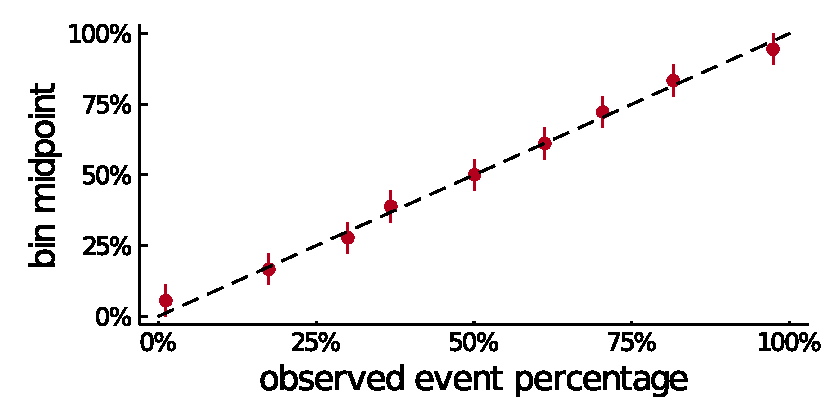
\includegraphics[width=1\linewidth]{plots/phylogeny_calibration.pdf}
  \caption{Calibration plot and how it works.}
\end{figure}

\subsection*{Including HLA linkage disequilibrium and codon covariation}

\begin{itemize}
  \item HLA linkage disequilibrium is accounted for by considering all HLA alleles
    of a sample at once.
  \item If strong correlations between HLA alleles: marginal posterior for both of them
    overlap with 0
  \item Codon covariation is not accounted for because we are mainly interested in HAMs.
  \item Model could be extended to include codon covariation by including them as additional
    predictors. This is possible because we use the horseshoe prior.
\end{itemize}

\subsection*{Including sparsity assumptions}

\begin{itemize}
  \item one of the recent advances in Bayesian inference: development of
    spacial priors to give model useful properties
  \item we expect most HLA coefficients to be 0, because no epitope spanning that region
    is presented on the cell surface, therefore no selection pressure and no association
    with possible replacements
  \item this is prior knowledge that should be incorporated in the model
  \item leads to better inferences because uncertainty of the regression coefficients
    does not propagate into observations.
  \item works by placing most probability mass very close to 0, but with large tails
    for non-zero coefficients.
  \item show formula
  \item global shrinkage parameter is very small and shrinks most coefficients to 0,
    local shrinkage parameter is very large and allows some coefficients to escape that 
    shrinkage
  \item prior can be specified in terms of expected number of non-zero coefficients
  \item in our case, degree of sparsity can be well estimated from the data because all
    replacements share the same global shrinkage parameter.
  \item useful addition for logistic regression models: regularized horseshoe
    to have some regularization for non-zero coefficients. this helps to deal with
    issues of separability and collinearity.
  \item effect of horseshoe prior compared to standard logistic regression model:
    refer to model testing section. In our benchmark, the horseshoe prior alone is more
    effective than the model with phylogeny.
  \item maybe include comparison of marginal posteriors with and without horseshoe prior
\end{itemize}

\subsection*{Including epitope prediction software}

\begin{itemize}
  \item Vast experimental data available.
  \item HAMs are much more likely to lie in known epitopes
  \item epitope prediction software works reasonably well and can be included into as
    input to a probabilitic model
  \item MHCFlurry is used for epitope prediction and Antigen processing prediction:
    Input matrix (dimensions: \#replacements x \#HLA alleles) contains a 1 if that
    position is either expected to be inside a predicted epitope or related to
    antigen processing, 0 otherwise
  \item uses some thresholds, but this is not so bad because we just use it as
    input for a probabilistic model. Maybe play around with different options?
    The Brumme paper uses some offsets for defining the region of known epitopes,
    maybe this does make a difference.
  \item including this kind of information can drastically improve predictive performance,
    as it is relevant external data.
  \item Bayesian inference allows us to include informationen from different sources in
    a consistent manner.
  \item this information may be imprecise or wrong, but the model is able to learn how much 
    to trust this data if parameterized correctly.
  \item epitope prediction / antigen processing escape is information about the expected
    degree of sparsity, i.e. some coefficients are more likely to be non-zero than others.
  \item can be included into the model by varying the local shrinkage parameter term.
  \item higher standard deviation of the local shrinkage parameters mean that
    it is more likely that this coefficient is non-zero.
  \item show formula
\end{itemize}

\subsection*{Partial pooling of 4-digit HLA alleles}

\begin{itemize}
  \item (this still has to be implemented, but should be a nice feature. If this
    is going to be too time consuming I can just leave it out)
  \item realized through allele group specific intercepts, e.g. HLA-B\*51:01 and 
  HLA-B\*51:03, ..., share a common intercept.
  \item show formula
\end{itemize}

\subsection*{Full model specification}
\begin{itemize}
  \item show all formulas
  \item all models were implementen in Stan. Code is available online in two versions:
  one optimized for readability, one optimized for speed with multithreading and GPU support
  \item data can be analyzed using a custom Julia package (tested on linux).
\end{itemize}

\subsection*{Prior justification}
\begin{itemize}
  \item justify priors, mostly based on the expected scales.
\end{itemize}

\section{Results and Discussion}

\thispagestyle{empty} % Removes page numbering from the first page
%----------------------------------------------------------------------------------------
%	ARTICLE CONTENTS
%----------------------------------------------------------------------------------------


\FloatBarrier

%----------------------------------------------------------------------------------------
%	REFERENCE LIST
%----------------------------------------------------------------------------------------
\phantomsection
\bibliographystyle{unsrt}
\bibliography{references}
%----------------------------------------------------------------------------------------

\end{document}